\chapter{Medical Image Segmentation}

\begin{itemize}
\item 
Start with general MS lesion segmentation
literature review.
\item What are the challenges and how could deep learning help to
overcome them?
\item Then literature using deep learning for segmentation.
Patch-based approaches for lesion segmentation, even if not MS lesions.
\item More recent approach are fully convolutional. Then explain my method
including the evaluation.
\end{itemize}

% TODO: Take MS motivation out into a separate MS part

Multiple sclerosis (MS) is an inflammatory and demyelinating disease of the
central nervous system with pathology that can be observed in vivo by magnetic
resonance imaging (MRI). MS is characterized by the formation of lesions,
primarily visible in the white matter on conventional MRI. Imaging biomarkers
based on the delineation of lesions, such as lesion load and lesion count, have
established their importance for assessing disease progression and treatment
effect. However, lesions vary greatly in size, shape, intensity and location,
which makes their automatic and accurate segmentation challenging.

\section{Related Work}

\subsection{MS Lesion Segmentation Methods}

Many automatic methods have been proposed for the segmentation of MS
lesions over the last two decades \citep{garcia2013}, which can be
classified into unsupervised and supervised methods. Unsupervised methods do not
require a labeled data set for training. Instead, lesions are identified as an
outlier class using, e.g., clustering methods
\citep{souplet2008,shiee2010} or generative models \citep{weiss2013}. In
addition to modelling MS lesions as a separate cluster, Lesion-TOADS
\citep{shiee2010} employs a topological and a statistical atlas to
produce a topology-preserving segmentation. Current supervised approaches
typically start with a large set of features, either predefined by the user
\citep{geremia2010} or gathered in a feature extraction step such as by deep
learning\citep{yoo2014}, which is followed by a separate training step with
labeled data to determine which set of features are the most important for
segmentation in the particular domain.
% For example, Yoo et al. \citep{yoo2014} proposed performing unsupervised
% learning of domain-specific features from image patches from unlabelled data
% using deep learning.
A recent breakthrough for automatic segmentation using deep learning comes from
the domain of cell membrane segmentation, in which Ciresan et al.
\citep{Ciresan2012} proposed to classify the centers of image patches directly
using a convolutional neural network (CNN) \citep{LeCun1998} without a dedicated
feature extraction step. Instead, features are learned indirectly within the
lower layers of the neural network during training, while the higher layers can
be regarded as performing the classification, which allows the learning of
features that are specifically tuned to the segmentation task. However, the time
required to train patch-based methods can make the approach infeasible when the
size and number of patches are large.

% TODO: can I add numerical values to it? Mostly my personal experience.

\subsection{Patch-based approaches using Deep Learning}

% TODO: Have to put Yoo and Ciresan here

\subsection{Fully Convolutional Approaches}

Recently, different CNN architectures
\citep{ronneberger2015,brosch2015,kang2014} have been proposed that are able
to feed through entire images, which removes the need to select representative
patches, eliminates redundant calculations where patches overlap, and therefore
scales up more efficiently with image resolution. Kang et al. introduced the
fully convolutional neural network (fCNN) for the segmentation of crowds in
surveillance videos \citep{kang2014}. However, fCNNs produce segmentations
of lower resolution than the input images due to the successive use of
convolutional and pooling layers, both of which reduce the dimensionality.
To predict segmentations of the same resolution as the input images, we recently
proposed using a 3-layer convolutional encoder network (CEN) \citep{brosch2015}
for MS lesion segmentation. The combination of convolutional \citep{LeCun1998}
and deconvolutional \citep{zeiler2011} layers allows our network to produce
segmentations that are of the same resolution as the input images. 

Another limitation of the traditional CNN is the trade-off between localization
accuracy, represented by lower-level features, and contextual information,
provided by higher-level features.
%
Ronneberger et al. \citep{ronneberger2015}
%
% found that increasing the depth of the
% CNN, and thereby increasing the size of the receptive field of a segmented voxel,
% increases the abstraction from the input data, which makes the segmentation
% method more robust to anatomical and intensity variations. They
%
proposed an 11-layer u-shaped network architecture called u-net,
% which leverages high-level and low-level features in order to predict
% segmentations that are both robust and accurate.
composed of a traditional contracting path (first half of the u), but augmented
with an expanding path (last half of the u), which replaces the pooling layers
of the contracting path with upsampling operations. To leverage both high- and
low-level features, shortcut connections are added between corresponding layers
of the two paths.
However,
% the successive application of convolutional, pooling, and
% unpooling layers reduces the size of the predicted segmentation by the size of
% the receptive field. This requires special handling of the border regions and
% limits the maximum size of the receptive field.
upsampling cannot fully compensate for the loss of resolution, and special
handling of the border regions is still required.

\section{Method}

We propose a new convolutional network architecture that combines the advantages
of a CEN \cite{brosch2015} and a u-net \cite{ronneberger2015}. Our network is
divided into two pathways, a traditional convolutional pathway, which consists
of alternating convolutional and pooling layers, and a deconvolutional pathway,
which consists of alternating deconvolutional and unpooling layers and predicts
the final segmentation. Similar to the u-net, we introduce shortcut connections
between layers of the two pathways. In contrast to the u-net, our network uses
deconvolution instead of upsampling in the expanding pathway and predicts
segmentations that have the same resolution as the input images and therefore
does not require special handling of the border regions.

\subsection{Solving Segmentation as an Optimization Problem}

In this paper, the task of segmenting MS lesions is defined as finding a
function $s$ that maps multi-modal images $I$, e.g., $I = (I_\text{FLAIR},
I_\text{T1})$, to corresponding lesion masks $S$. Given a set of
training images $I_n$, $n \in \N$, and corresponding segmentations $S_n$, we
model finding an appropriate function for segmenting MS lesions as an
optimization problem of the following form
\begin{equation}
\hat{s} = \arg \min_{s \in \mathcal{S}} \sum_n E(S_n, s(I_n)),
\label{eq:segprob}
\end{equation}
where $\mathcal{S}$ is the set of possible segmentation functions, and $E$ is an
error measure that calculates the dissimilarity between ground truth
segmentations and predicted segmentations.

\subsection{Model Architecture}

The set of possible segmentation functions, $\mathcal{S}$, is modeled by the
convolutional encoder network with shortcut connections (CEN-s) illustrated in
Fig.~\ref{fig:network}. A CEN-s is a type of convolutional neural network (CNN)
\cite{LeCun1998} that is divided into two interconnected pathways, the
convolutional pathway and the deconvolutional \cite{zeiler2011} pathway. The
convolutional pathway consists of alternating convolutional and pooling layers.
The input layer of the convolutional pathway is composed of the image voxels
$x^{(0)}_i(\vect{p})$, $i \in [1, C]$, where $i$ indexes the modality or input
channel, $C$ is the number of modalities or channels, and $\vect{p} \in \N^3$
are the coordinates of a particular voxel. The convolutional layers
automatically learn a feature hierarchy from the input images. A convolutional
layer is a deterministic function of the following form
\begin{equation}
x^{(l)}_j = \max \Bigg(0, \sum_{i=1}^C\tilde{w}^{(l)}_{\text{c},ij}*x^{(l-1)}_i
+ b^{(l)}_j\Bigg),
\end{equation}
where $l$ is the index of a convolutional layer, $x^{(l)}_j$, $j \in [1,F]$,
denotes the feature map corresponding to the trainable convolution filter
$w^{(l)}_{\text{c},ij}$, $F$ is the number of filters of the current layer,
$b^{(l)}_j$ are trainable bias terms, $*$ denotes valid convolution, and
$\tilde{w}$ denotes a flipped version of $w$. A convolutional layer is followed
by an average pooling layer \cite{scherer2010} that halves the number
of units in each dimension by calculating the average of each block of
\num{2x2x2} units per channel.

\begin{figure}[tb]
\centering
\begin{tikzpicture}[
  node distance=0.75cm and 0.65cm,
  font=\footnotesize,
  conv/.style={green!60!black,-latex,thick},
  conv2/.style={green!60!black,latex-latex,thick},
  deconv/.style={-latex,blue!40!black,thick},
  %pooling/.style={-latex,red!60!black,thick,dashed},
  %unpooling/.style={-latex,brown!60!black,thick,dashed},
  pooling/.style={-latex,green!60!black,thick,dashed},
  unpooling/.style={-latex,blue!40!black,thick,dashed},
  channel/.style args={#1 and #2}{draw, fill=lightgray, inner sep=0pt,
      minimum width=#1, minimum height=#2}
]

% \tikzstyle{channel}=[draw,minimum width=64pt,fill=lightgray,inner
% sep=0pt,minimum height=#1]

% Network

\begin{scope}[local bounding box=network]
\node[channel=64pt and 3pt,pin=270:Input images] (inputs) {};
\node[channel=60pt and 16pt,above=of inputs] (clayer1) {};
\node[channel=30pt and 16pt,above=of clayer1] (pooling1) {};

\node[channel=64pt and 1pt,right=of inputs,pin=270:Segmentations] (outputs) {};
\node[channel=60pt and 16pt] (dlayer1) at (clayer1-|outputs) {};
\node[channel=30pt and 16pt,above=of dlayer1] (dpooling1) {};

\node[fit=(pooling1)(dpooling1),inner sep = 0pt] (pooling) {};
\node[channel=26pt and 16pt,above=of pooling] (clayer2) {};
\end{scope}

\draw[conv] (inputs)--node[left] {$w^{(1)}_\text{c}$} (clayer1);
\draw[pooling] (clayer1)--node[left] {} (pooling1);
\draw[conv] (pooling1)--node[left] {$w^{(3)}_\text{c}$} (clayer2);
\draw[deconv] (clayer2)--node[right=5pt] {$w^{(3)}_\text{d}$} (dpooling1);
\draw[unpooling] (dpooling1)--node[right] {} (dlayer1);
\draw[deconv] (dlayer1)--node[right] {$w^{(1)}_\text{d}$} (outputs);
\draw[deconv] (clayer1)--node[anchor=188,inner sep=10pt]
{$w^{(1)}_\text{s}$}(outputs);

% Part labels

\node[left=1pt of inputs] {$x^{(0)}$};
\node[left=1pt of clayer1] {$x^{(1)}$};
\node[left=1pt of pooling1] {$x^{(2)}$};
\node[left=1pt of clayer2] {$x^{(3)}$};

\node[right=1pt of outputs] {$y^{(0)}$};
\node[right=1pt of dlayer1] {$y^{(1)}$};
\node[right=1pt of dpooling1] {$y^{(2)}$};
\node[right=1pt of clayer2] {$y^{(3)}$};

% Layers

\draw[decorate,decoration={brace,raise=30pt}] (inputs.south west)
--node[left=35pt,align=center] (convl) {Convolutional\\ layer} (inputs.south
west|-clayer1.north west);

\draw[decorate,decoration={brace,raise=22pt}] (clayer1.south west)
--node[left=27pt,align=center] {Pooling\\ layer} (clayer1.south
west|-pooling1.north west);

\draw[decorate,decoration={brace,raise=25pt}] (pooling1.south west)
--node[left=30pt,align=center] {Convolutional\\ layer} (clayer2.north
west-|pooling1.south west);

\draw[decorate,decoration={brace,raise=30pt,mirror}] (outputs.south east)
--node[right=35pt,align=center] {Deconvolutional\\ layer with shortcut}
 (dlayer1.north east-|outputs.south east);

\draw[decorate,decoration={brace,raise=22pt,mirror}] (dlayer1.south east)
--node[right=27pt,align=center] {Unpooling\\ layer}
(dpooling1.north east-|dlayer1.south east);

\draw[decorate,decoration={brace,raise=25pt,mirror}] (dpooling1.south east)
--node[right=30pt,align=center] {Deconvolutional\\ layer}
(clayer2.north east-|dpooling1.south east);

% Legend

\begin{scope}[local bounding box=ghost,opacity=0]
\path[conv] node (conv) {convolution} [draw] (conv.west)
++(left:0.5)--++(right:0.5);

\path[pooling] node[right=0.8 of conv] (pool) {pooling} [draw] (pool.west)
++(left:0.5)--++(right:0.5);

\path[deconv] node[right=0.8 of pool] (dconv) {deconvolution} [draw]
(dconv.west) ++(left:0.5)--++(right:0.5);

\path[unpooling] node[right=0.8 of dconv] (unpool) {unpooling} [draw]
(unpool.west) ++(left:0.5)--++(right:0.5);
\end{scope}

\begin{scope}[local bounding box=ghost2,
    shift={($(network.south)-(ghost.north)$)},xshift=2pt,yshift=-7pt]

\path[conv] node (conv) {convolution} [draw] (conv.west)
++(left:0.5)--++(right:0.5);

\path[pooling] node[right=0.8 of conv] (pool) {pooling} [draw] (pool.west)
++(left:0.5)--++(right:0.5);

\path[deconv] node[right=0.8 of pool] (dconv) {deconvolution} [draw]
(dconv.west) ++(left:0.5)--++(right:0.5);

\path[unpooling] node[right=0.8 of dconv] (unpool) {unpooling} [draw]
(unpool.west) ++(left:0.5)--++(right:0.5);
\end{scope}

% Stack of CRBMs

\begin{scope}[local bounding box=dbn]
\node[channel=64pt and 3pt, left=6cm of inputs,pin=270:Input images] (rinputs)
{}; 
\node[channel=60pt and 16pt,above=of rinputs] (rclayer1) {};
\node[channel=30pt and 16pt,above=of rclayer1] (rpooling1) {};
\node[channel=26pt and 16pt,above=of rpooling1] (rclayer2) {};
\end{scope}

\draw[conv2] (rinputs)--node[left] {$\hat{w}^{(1)}$} (rclayer1);
\draw[pooling] (rclayer1)--node[right] {pooling} (rpooling1);
\draw[conv2] (rpooling1)--node[left] {$\hat{w}^{(2)}$} (rclayer2);

\node[left=1pt of rinputs] {$v^{(1)}$};
\node[left=1pt of rclayer1] {$h^{(1)}$};
\node[left=1pt of rpooling1] {$v^{(2)}$};
\node[left=1pt of rclayer2] {$h^{(2)}$};

\draw[decorate,decoration={brace,raise=5pt,mirror}] (rinputs.south east)
--node[right=10pt,align=center] (crbm) {convRBM$_1$} (rinputs.south
east|-rclayer1.north east);

\draw[decorate,decoration={brace,raise=5pt,mirror}] (rpooling1.south east)
--node[right=10pt,align=center] {convRBM$_2$} (rclayer2.north
east-|rpooling1.south east);

% \node[above=10pt of dbn,align=center] {Stack of Convolutional\\ Restricted
% Boltzmann Machines};
% \node[above=10pt of network] {Convolutional Encoder Network};

\node[above=15pt of dbn,align=center,font=\normalsize] {Pre-training};
\node[above=15pt of network,font=\normalsize] {Fine-tuning};

% \draw[->] (crbm.east|-dbn)-- node[above=2pt] {convert} 
% node[above,align=center]
% {$w_\text{c}^{(1)} = w^{(1)}$ \\
%  $w_\text{c}^{(2)} = w^{(2)}$ \\
%  $w_\text{d}^{(2)} = w^{(2)}$ \\
%  $w_\text{d}^{(1)} = 0.5w^{(1)}$ \\
%  $w_\text{s}^{(1)} = 0.5w^{(1)}$}
% (convl.west|-network);

%\draw (network.north west) rectangle (network.south east);
%\draw (ghost.north west) rectangle (ghost.south east);
%\draw (ghost2.north west) rectangle (ghost2.south east);

%\path[pooling] node (pool) at (-3,-1) {convolution};
%\draw[pooling] (conv.west) ++(left:0.5)--++(right:0.5);

%\draw[conv] (-3,-1)-- +(right:0.5) node[right] {convolution};
%\draw[pooling] (-0.5,-1)-- +(right:0.5) node[right] {pooling};
%\draw[deconv] (2,-1)-- +(right:0.5) node[right] {deconvolution};
%\draw[unpooling] (4.5,-1)-- +(right:0.5) node[right] {unpooling};

%\draw[pooling] (0,-1.5)-- +(right:0.5) node[right] {pooling};
%\draw[deconv] (0,-2)-- +(right:0.5) node[right] {deconvolution};
%\draw[unpooling] (0,-2.5)-- +(right:0.5) node[right] {unpooling};

\end{tikzpicture}

\caption[Pre-training and fine-tuning of the 7-layer convolutional encoder
network with shortcut]{Pre-training and fine-tuning of the 7-layer convolutional
encoder network with shortcut that we used for our experiments. Pre-training is
performed on the input images using a stack of convolutional RBMs. The
pre-trained weights and bias terms are used to initialize a convolutional
encoder network, which is fine-tuned on pairs of input images, $x^{(0)}$, and
segmentations, $y^{(0)}$.}

\label{fig:network}
\end{figure}

The deconvolutional pathway consists of alternating deconvolutional and
unpooling layers with shortcut connections to the corresponding
convolutional layers. The first deconvolutional layer uses the extracted
features of the convolutional pathway to calculate abstract segmentation
features
\begin{equation}
y^{(L-1)}_i = \max\Bigg(0, \sum_{j=1}w^{(L)}_{\text{d},ij}\circledast
y^{(L)}_j + c^{(L-1)}_{i}\Bigg),
\end{equation}
where $y^{(L)} = x^{(L)}$, $L$ denotes the number of layers of the convolutional
pathway, $w^{(L)}_{\text{d},ij}$ and $c^{(L-1)}_i$ are trainable parameters of
the deconvolutional layer, and $\circledast$ denotes full convolution. Subsequent
deconvolutional layers use the activations of the previous layer
and corresponding convolutional layer to calculate more localized segmentation
features
% \begin{multline}
% y^{(l)}_i = \max\Bigg(0, \sum_{j=1}\Big(w^{(l+1)}_{\text{d},ij}\circledast
% y^{(l+1)}_j\\
% + w^{(l+1)}_{\text{s},ij}\circledast x^{(l+1)}_j\Big) +
% c^{(l)}_i\Bigg)
% \end{multline}
\begin{multline}
y^{(l)}_i = \max\Bigg(0, 
\sum_{j=1}w^{(l+1)}_{\text{d},ij}\circledast y^{(l+1)}_j\\
+ \sum_{j=1} w^{(l+1)}_{\text{s},ij}\circledast x^{(l+1)}_j +
c^{(l)}_i\Bigg),
\end{multline}
where $l$ is the index of a deconvolutional layer with shortcut, and
$w^{(l+1)}_{\text{s},ij}$ are the shortcut filter kernels connecting the
activations of the convolutional pathway with the activations of the
deconvolutional pathway. The last deconvolutional layer integrates the low-level
features extracted by the first convolutional layer with the high-level features
from the previous layer to calculate a probabilistic lesion mask
\begin{equation}
y^{(0)}_1 = \sigm\Bigg(\sum_{j=1}\Big(w^{(1)}_{\text{d},1j}\circledast
y^{(1)}_j +
w^{(1)}_{\text{s},1j}\circledast x^{(1)}_j\Big) + c^{(0)}_1\Bigg),
\end{equation}
where $\sigm(z)$ denotes the sigmoid function defined as $\sigm(z) = (1 +
\exp(-z))^{-1}, z \in \R$. To obtain a binary lesion mask from the probabilistic
output of our model, we chose a fixed threshold such that the mean Dice
similarity coefficient \cite{dice1945} is maximized on the training set
and used the same threshold for the evaluation on the test set.

\begin{comment}
The set of possible segmentation functions is modeled by the convolutional
encoder network illustrated in Fig.~\ref{fig:network}. Our network consists of
three layers: an input layer, a convolutional layer, and a deconvolutional
layer. The input layer is composed of the image voxels $x^{(1)}_i(\vect{p})$, $i
\in [1, C], C \in \N$, where $i$ indexes the modality, $C$ is the number of
modalities, and $\vect{p} \in \R^3$ are the coordinates of a particular voxel.
The convolutional layer automatically learns features from the input images. It
is a deterministic function of the following form
\begin{equation}
y^{(1)}_j = \max \left(0, \sum_{i=1}^{C}\tilde{w}^{(1)}_{ij}*x^{(1)}_i +
b^{(1)}_j\right)
\end{equation}
where $y^{(1)}_j, j \in [1, F], F \in \N$, denotes the feature map corresponding
to the trainable convolution filter $w^{(1)}_{ij}$, $F$ is the number of
filters, $b_j$ is a trainable bias term, $*$ denotes valid convolution, and
$\tilde{w}$ denotes a flipped version of $w$. The deconvolutional layer uses the
extracted features to calculate a probabilistic lesion mask as follows
\begin{equation}
y^{(2)} = \sigm\left(\sum_{j=1}^Fw^{(2)}_{j}\circledast x^{(2)}_j +
b^{(2)}\right)
\end{equation}
where $x^{(2)}_j = y^{(1)}_j$, $w^{(2)}_j$ and $b^{(2)}$ are trainable
parameters, $\circledast$ denotes full convolution, and $\sigm(z)$ denotes the
sigmoid function defined as $\sigm(z) = (1 + \exp(-z))^{-1}, z \in \R$. To
obtain a binary lesion mask from the probabilistic output of our model, we chose
a fixed threshold such that the mean Dice similarity coefficient is
maximized on the training set.
\end{comment}

% \begin{itemize}
% \item Parameters can be learned by minimizing the error $E$ on the training set
% \item Minimization requires calculation of gradient
% \item Derive the gradient, also with new notation, multiple layers and short
% cuts
% \end{itemize}

\subsection{Gradient Calculation}

The parameters of the model can be efficiently learned by minimizing the error
$E$ on the training set, which requires the calculation of the gradient of $E$
with respect to the model parameters \cite{LeCun1998}. Typically, neural
networks are trained by minimizing the sum of squared differences (SSD)
\begin{equation}
% Error function
E = \frac{1}{2}\sum_{\vect{p}}\left(S(\vect{p}) -
y^{(2)}(\vect{p})\right)^2.
\end{equation}
The partial derivatives of the error with respect to the model parameters can be
calculated using the delta rule and are given by 
% $\Delta w^{(l)}_{\text{d},ij} =
% \delta^{(l-1)}_{\text{d},i} * \tilde{y}^{(l)}_j$, $\Delta w^{(l)}_{\text{s},ij}
% = \delta^{(l-1)}_{\text{d},i} * \tilde{x}^{(l)}_j$, $\Delta
% w^{(l)}_{\text{c},ij} = x^{(l-1)}_i * \tilde{\delta}^{(l)}_{\text{c},j}$
\begin{align}
\label{eq:dEd}
% Deconvolutional filters
\frac{\partial E}{\partial w^{(l)}_{\text{d},ij}} &=
\delta^{(l-1)}_{\text{d},i} * \tilde{y}^{(l)}_j, &
% Deconvolutional bias
\frac{\partial E}{\partial c^{(l)}_i} &= \sum_{\vect{p}}
\delta^{(l)}_{\text{d},i}(\vect{p}), \\
\label{eq:dEs}
% Shortcut filters
\frac{\partial E}{\partial w^{(l)}_{\text{s},ij}}
 &= \delta^{(l-1)}_{\text{d},i} * \tilde{x}^{(l)}_j, \\
 \label{eq:dEc}
% Convolutional filters
\frac{\partial E}{\partial w^{(l)}_{\text{c},ij}} 
&= x^{(l-1)}_i * \tilde{\delta}^{(l)}_{\text{c},j},\text{ and}&
% Convolutional bias
\frac{\partial E}{\partial b^{(l)}_i} &= \sum_{\vect{p}}
\delta^{(l)}_{\text{c},i}(\vect{p}).
\end{align}
For the first layer, $\delta^{(0)}_{\text{d},1}$ can be calculated by
\begin{equation}
% Delta update
\delta^{(0)}_{\text{d},1} = \big(y^{(0)}_1
-S\big)y^{(0)}_1\big(1-y^{(0)}_1\big).
\label{eq:delta0}
\end{equation}
The derivatives of the error with respect to the parameters of the other layers
can be calculated by applying the chain rule of partial derivatives, which
yields to
\begin{align}
\label{eq:deltad}
% Delta update of deconvolutional layer
\delta^{(l)}_{\text{d},j} &=
\big(\tilde{w}^{(l)}_{\text{d},ij}*\delta^{(l-1)}_{\text{d},i}\big)\I\big(y^{(l)}_j
> 0\big),\\
\label{eq:deltac}
% Delta update of convolutional layer
\delta^{(l)}_{\text{c},i} &=
\big(w^{(l+1)}_{\text{c},ij}\circledast\delta^{(l+1)}_{\text{c},j}\big)\I\big(x^{(l)}_i
> 0\big),
\end{align}
where $l$ is the index of a deconvolutional or convolutional layer,
$\delta^{(L)}_{\text{c},i} = \delta^{(L)}_{\text{d},j}$, and $\I(z)$ denotes the
indicator function defined as $1$ if the predicate $z$ is true and $0$
otherwise. If a layer connected through a shortcut,
$\delta^{(l)}_{\text{c},j}$ needs to be adjusted by propagating the error back
through the shortcut connections. In this case, $\delta^{(l)}_{\text{c},j}$ is
calculated by
\begin{equation}
% Delta update convolutional with shortcut
\delta^{(l)}_{\text{c},j} =
\big(\delta^{(l)}_{\text{c},j}{}'+
\tilde{w}^{(l)}_{\text{s},ij}*\delta^{(l-1)}_{\text{d},i}\big)\I\big(x^{(l)}_j
> 0\big),
\label{eq:deltas}
\end{equation}
where $\delta^{(l)}_{\text{c},j}{}'$ denotes the activation of unit
$\delta^{(l)}_{\text{c},j}$ before taking the shortcut connection into account.

% Introduce new objective function and it's gradient

The sum of squared differences is a good measure of classification accuracy, if
the two classes are fairly balanced. However, if one class contains vastly more
samples, as is the case for lesion segmentation, the error measure is dominated
by the majority class and consequently, the neural network would learn to ignore
the minority class. To overcome this problem, we use a combination of
sensitivity and specificity, which can be used together to measure
classification performance even for vastly unbalanced problems. More precisely,
the final error measure is a weighted sum of the mean squared difference of the
lesion voxels (sensitivity) and non-lesion voxels (specificity), reformulated to
be error terms:
\begin{multline} 
E = r\frac{\textstyle\sum_{\vect{p}} \left(S(\vect{p}) -
y^{(2)}(\vect{p})\right)^2 S(\vect{p})}{\textstyle\sum_{\vect{p}} S(\vect{p})}
\\
 + (1-r)\frac{\textstyle\sum_{\vect{p}} \left(S(\vect{p}) -
y^{(2)}(\vect{p})\right)^2 \big(1 - S(\vect{p})\big)}{%
\textstyle\sum_{\vect{p}}\big(1 - S(\vect{p})\big)}.
\end{multline}
We formulate the sensitivity and specificity errors as squared errors in order
to yield smooth gradients, which makes the optimization more robust. The
sensitivity ratio $r$ can be used to assign different weights to the two terms.
Due to the large number of non-lesion voxels, weighting the specificity error
higher is important, but based on preliminarily experimental results, the
algorithm is stable with respect to changes in $r$, which largely affects the
threshold used to binarize the probabilistic output. In all our experiments, a
sensitivity ratio between $0.10$ and $0.01$ yielded very similar results.

To train our model, we must compute the derivatives of the modified objective
function with respect to the model parameters. Equations
\ref{eq:dEd}--\ref{eq:dEc} and \ref{eq:deltad}--\ref{eq:deltas} are a
consequence of the chain rule and independent of the chosen similarity measure.
Hence, we only need to derive the update rule for $\delta^{(0)}_{\text{d},1}$.
With $\alpha = 2r (\sum_{\vect{p}}S(\vect{p}))^{-1}$ and $\beta = 2(1 -
r)(\sum_{\vect{p}}(1 - S(\vect{p})))^{-1}$, we can rewrite $E$ as
\begin{align}
% \nonumber
% E =& \frac{1}{2}\sum_{\vect{p}}\Big(S(\vect{p})-y^{(0)}_1(\vect{p})\Big)^2 
% \alpha S(\vect{p})\\
% &+\frac{1}{2}\sum_{\vect{p}}\Big(S(\vect{p})-y^{(0)}_1(\vect{p})\Big)^2
% \beta(1-S(\vect{p}))\\
E=& \frac{1}{2}\sum_{\vect{p}}\big(\alpha S(\vect{p}) +
\beta(1-S(\vect{p}))\big)\Big(S(\vect{p})-y^{(0)}_1(\vect{p})\Big)^2.
\end{align}
%
Our objective function is similar to the SSD, with an additional multiplicative
term applied to the squared differences. The additional factor is constant with
respect to the model parameters. Consequently, $\delta^{(0)}_{\text{d},1}$ can
be derived analogously to the SSD case, and the new factor is simply carried
over:
\begin{equation} 
\delta^{(0)}_{\text{d},1} = \big(\alpha S + \beta (1 - S)\big)\big(y^{(0)}_1 -
S\big) y^{(0)}_1 \big(1 - y^{(0)}_1\big).
\end{equation}

% The update for $\delta^{(0)}_{\text{d},1}$ can be derived analogously to the SSD
% case, and is given by
% \begin{equation} 
% \delta^{(0)}_{\text{d},1} = \big(\alpha S + \beta (1 - S)\big)\big(y^{(0)}_1 -
% S\big) y^{(0)}_1 \big(1 - y^{(0)}_1\big)
% \end{equation}
% where $\alpha = 2r (\sum_{\vect{p}}S(\vect{p}))^{-1}$ and $\beta = 2(1 -
% r)(\sum_{\vect{p}}(1 - S(\vect{p})))^{-1}$.

\subsection{Training}
% Initialize training

At the beginning of the training procedure, the model parameters need to be
initialized and the choice of the initial parameters can have a big impact on
the learned model \cite{sutskever2013}. In our experiments, we found that
initializing the model using pre-training \cite{hinton2006c} on the input images
was required in order to be able to fine-tune the model using the ground truth
segmentations without getting stuck in an early local minimum. Pre-training can
be performed layer by layer \cite{Hinton2006b} using a stack of convolutional
restricted Boltzmann machines (convRBMs) \cite{lee2009} (see
Fig.~\ref{fig:network}), thereby avoiding the potential problem of vanishing or
exploding gradients \cite{hochreiter1991}. The first convRBM is trained on the
input images, while subsequent convRBMs are trained on the hidden activations of
the previous convRBM. After all convRBMs have been trained, the model parameters
of the CEN-s can be initialized as follows (showing the first convolutional and
the last deconvolutional layers only, see Fig.~\ref{fig:network})
\begin{align}
w_{\text{c}}^{(1)} &= \hat{w}^{(1)}, &
w_{\text{d}}^{(1)} &= 0.5\hat{w}^{(1)}, &
w_{\text{s}}^{(1)} &= 0.5\hat{w}^{(1)} \\
b^{(1)} &= \hat{b}^{(1)}, &
c^{(0)} &= \hat{c}^{(1)},
\end{align}
where $\hat{w}^{(1)}$ are the filter weights, $\hat{b}^{(1)}$ are the hidden
bias terms, and $\hat{c}^{(1)}$ are the visible bias terms of the first convRBM.
% Alternatively, the bias terms can be initialized with zero and the
% filter weights are initialized using random values that are drawn from a
% distribution such that the variance of the activations of the layer units
% remains roughly the same throughout all layers. This can be achieved by drawing
% samples from the normal distribution $\mathcal{N}(0, \sigma)$, where $\sigma =
% \sqrt{2/N}$, and $N$ denotes the number of incoming connections for one unit.
% The influence of the initialization strategy on the learned model is analyzed in
% Section~??.

Recap that finding a learning rate can be challenging. Tried different methods
for setting the learning rate. In our initial experiments, networks obtained by
training with AdaDelta, RMSprop, and Adam performed comparably well, but
AdaDelta was the most robust to the choice of hyperparameters, so we used
AdaDelta for all results reported.

% A major challenge for gradient-based optimization methods is the choice of an
% appropriate learning rate. Classic stochastic gradient descent \cite{LeCun1998}
% uses a fixed or decaying learning rate, which is the same for all parameters of
% the model. However, the partial derivatives of parameters of different layers
% can vary substantially in magnitude, which can require different learning rates.
% In recent years, there has been an increasing interest in developing methods for
% automatically choosing independent learning rates. Most methods (e.g., AdaGrad
% \cite{duchi2011}, AdaDelta \cite{zeiler2012}, RMSprop
% \cite{dauphin2015}, and Adam \cite{kingma2014}) collect different
% statistics of the partial derivatives over multiple iterations and use this
% information to set an adaptive learning rate for each parameter. This is
% especially important for the training of deep networks, where the optimal
% learning rates often differ greatly for each layer. In our initial experiments,
% networks obtained by training with AdaDelta, RMSprop, and Adam performed
% comparably well, but AdaDelta was the most robust to the choice of
% hyperparameters, so we used AdaDelta for all results reported.

% Second-order methods, like
% Hessian-free optimization [??], do not require a learning rate. Instead, a step
% towards the minimum of a quadratic approximation of the error function (or a
% semi positive definite approximation thereof) is performed in each iteration.
% Calculation of one update is much more costly for second-order methods, but it
% also performs much more progress and navigates valleys of ``pathological
% curvature'' more efficiently, which reduces the number of epochs required to
% train the model. For more details about the aforementioned methods, the reader
% is referred to the relevant papers.

\sisetup{separate-uncertainty=true,detect-weight=true,detect-inline-weight=math}


% \uselengthunit{in}\printlength{\textwidth} = 4.8041 in
% \uselengthunit{mm}\printlength{\textwidth} = 121.99854 mm

%\subsection{Data Sets and Pre-processing}

% TODO: How was split determined: all scans of the same patient and scanning
% site were put in the same group

% TODO: Why did I choose Lesion-TOADS?

\section{Evaluation with the State-of-the-art}

To allow for a direct comparison with state-of-the-art lesion segmentation
methods, we evaluated our method on the FLAIR, T1-, and T2-weighted MRIs of the
20 publicly available labeled cases from the MS lesion segmentation challenge
2008 \cite{styner20083d}, which we downsampled from the original isotropic voxel
size of \SI{0.5}{\cubic\milli\metre} to an isotropic voxel size of
\SI{1.0}{\cubic\milli\metre}. In addition, we evaluated our method on an
in-house data set from an MS clinical trial of 500 subjects split equally into
training and test sets. The images were acquired from 45 different scanning
sites. For each subject, the data set contains T2- and PD-weighted MRIs with a
voxel size of \SI{0.937x0.937x3.000}{\milli\metre}. The main preprocessing steps
included rigid intra-subject registration, brain extraction, intensity
normalization, and background cropping.

We used a CEN with 32 filters and filter sizes of \num{9x9x9} and \num{9x9x5}
voxels for the challenge and in-house data sets, respectively. Training on a
single GeForce GTX 780 graphics card took between 6 and 32 hours per model
depending on the training set size. However, once the network is trained,
segmentation of trimodal 3D volumes with a resolution of, e.g.,
\num{159x201x155} voxels can be performed in less than one second. As a
rough\footnote{Ciresan et al. used a more complex network that is composed of 11
layers. However, their network was trained on much smaller images, which roughly
compensates for the increased complexity.} comparison, Ciresan et al.
\cite{Ciresan2012} reported that their patch-based method required 10 to 30
minutes to segment a single 2D image with a resolution of \num{512x512} voxels
using four graphics cards, which demonstrates the large speed-ups gained by
processing entire volumes.

\begin{figure}[tb]
\centering
\small
\def\MRIwidth{0.15\textwidth}

\begin{tikzpicture} 
\tikzstyle{leftlabel}=[rotate=90, align=center,overlay,above]

\matrix [matrix of nodes, nodes={anchor=center, inner sep=1pt}] {
        &[4pt] FLAIR & T1w & T2w & Ground truth & Our method \\[4pt]
\node[leftlabel] {CHB\,07\\(DSC\,=\,\SI{60.58}{\percent})}; &
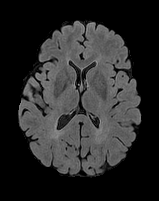
\includegraphics[width=\MRIwidth]{figures/MICCAI2015_CHB07-FLAIR-s88} &
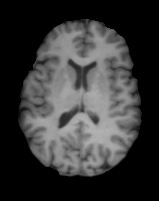
\includegraphics[width=\MRIwidth]{figures/MICCAI2015_CHB07-T1w-s88} &
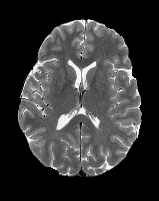
\includegraphics[width=\MRIwidth]{figures/MICCAI2015_CHB07-T2w-s88} &
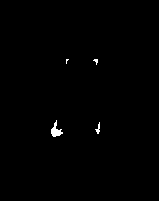
\includegraphics[width=\MRIwidth]{figures/MICCAI2015_CHB07-gold-s88} &
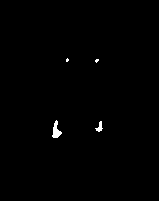
\includegraphics[width=\MRIwidth]{figures/MICCAI2015_CHB07-pred-s88} \\
\node[leftlabel] {CHB\,04\\(DSC\,=\,\SI{61.37}{\percent})}; &
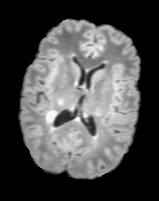
\includegraphics[width=\MRIwidth]{figures/MICCAI2015_CHB04-FLAIR-s85} &
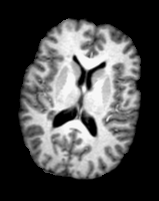
\includegraphics[width=\MRIwidth]{figures/MICCAI2015_CHB04-T1w-s85} &
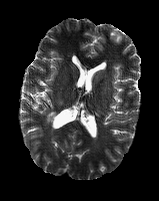
\includegraphics[width=\MRIwidth]{figures/MICCAI2015_CHB04-T2w-s85} &
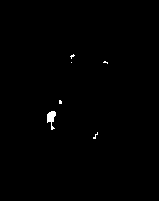
\includegraphics[width=\MRIwidth]{figures/MICCAI2015_CHB04-gold-s85} &
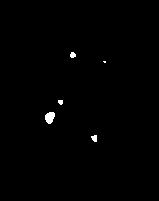
\includegraphics[width=\MRIwidth]{figures/MICCAI2015_CHB04-pred-s85} \\
\node[leftlabel] {UNC\,09\\(DSC\,=\,\SI{9.01}{\percent})}; &
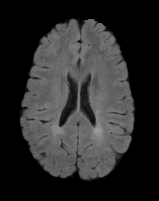
\includegraphics[width=\MRIwidth]{figures/MICCAI2015_UNC09-FLAIR-s89} &
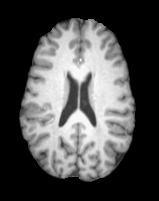
\includegraphics[width=\MRIwidth]{figures/MICCAI2015_UNC09-T1w-s89} &
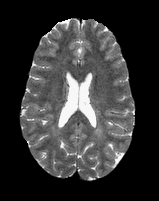
\includegraphics[width=\MRIwidth]{figures/MICCAI2015_UNC09-T2w-s89} &

\includegraphics[width=\MRIwidth]{figures/MICCAI2015_UNC09-gold-s89} &
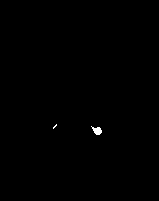
\includegraphics[width=\MRIwidth]{figures/MICCAI2015_UNC09-pred-s89} \\
};
\end{tikzpicture}

\caption[Example segmentations of our method for three different subjects from
the challenge data set]{Example segmentations of our method for three different
subjects from the challenge data set. Our method performed well and consistently
despite the large contrast differences seen between the first two rows. In the
third row, our method also segmented lesions that have similar contrast, but
these regions had not been identified as lesions by the manual rater, which
highlights the difficulty in distinguishing focal lesions from diffuse damage,
even for experts.}

\label{fig:segmentation}
\end{figure}

We evaluated our method on the challenge data set using 5-fold
cross-valida\-tion and calculated the true positive rate (TPR), positive
predictive value (PPV), and Dice similarity coefficient (DSC) between the
predicted segmentations and the resampled ground truth.
Figure~\ref{fig:segmentation} shows a comparison of three subjects from the
challenge data set. The first two rows show the FLAIR, T1w, T2w, ground truth
segmentations, and predicted segmentations of two subjects with a DSC of
\SI{60.58}{\percent} and \SI{61.37}{\percent}. Despite the large contrast
differences between the two subjects, our method performed well and
consistently, which indicates that our model was able to learn features that are
robust to a large range of intensity variations. The last row shows a subject
with a DSC of \SI{9.01}{\percent}, one of the lowest DSC scores from the data
set. Our method segmented lesions that have similar contrast to the other two
subjects, but these regions were not classified as lesions by the manual rater.
This highlights the difficulty of manual lesion segmentation, as the difference
between diffuse white matter pathology and focal lesions is often indistinct. A
quantitative comparison of our method with other state-of-the-art methods is
summarized in Table~\ref{tab:state}. Our method outperforms the winning method
(Souplet et al. \cite{souplet2008}) of the MS lesion segmentation challenge 2008
and the currently best unsupervised method reported on that data set (Weiss et
al. \cite{weiss2013}) in terms of mean TPR and PPV. Our method performs
comparably to a current method (Geremia et al. \cite{geremia2010}) that uses a
carefully designed set of features specifically designed for lesion
segmentation, despite our method having learned its features solely from a
relatively small training set.

\begin{table}[tb]
\def\tabspace{12pt}

\caption[Comparison of our method with state-of-the-art lesion segmentation
methods]{Comparison of our method with state-of-the-art lesion segmentation
methods in terms of mean TPR, PPV, and DSC. Our method performs comparably to
the best methods reported on the MS lesion segmentation challenge data set.}

\label{tab:state}
\centering
\begin{tabular}{l%
@{\hspace{\tabspace}}S[table-format=2.2]
@{\hspace{\tabspace}}S[table-format=2.2]
@{\hspace{\tabspace}}S[table-format=2.2]
}
\toprule
Method & {TPR} & {PPV} & {DSC} \\ 
\midrule
Souplet et al. \cite{souplet2008} & 20.65 & 30.00 & {---} \\ 
Weiss et al. \cite{weiss2013} & 33.00 & 36.85 & 29.05 \\ 
Geremia et al. \cite{geremia2010} & 39.85 & 40.35 & {---}  \\
Our method & 39.71 & 41.38 & 35.52 \\
\bottomrule
\end{tabular}
\end{table}

To evaluate the impact of the training set size on the segmentation performance,
we trained our model on our in-house data set with a varying number of training
samples and calculated the mean DSC on the training and test sets as illustrated
in Fig.~\ref{fig:bioms}. For small training sets, there is a large difference
between the DSCs on the training and test sets, which indicates that the
training set is too small to learn a representative set of features. At around
100 samples, the model becomes stable in terms of test performance and the small
difference between training and test DSCs, indicating that overfitting of the
training data is no longer occurring. With 100 training subjects, our method
achieves a mean DSC on the test set of \SI{57.38}{\percent}, which shows that
the segmentation accuracy can be greatly improved compared to the results on the
challenge data set, when a representative training set is available.

\begin{figure}[tb]
\centering
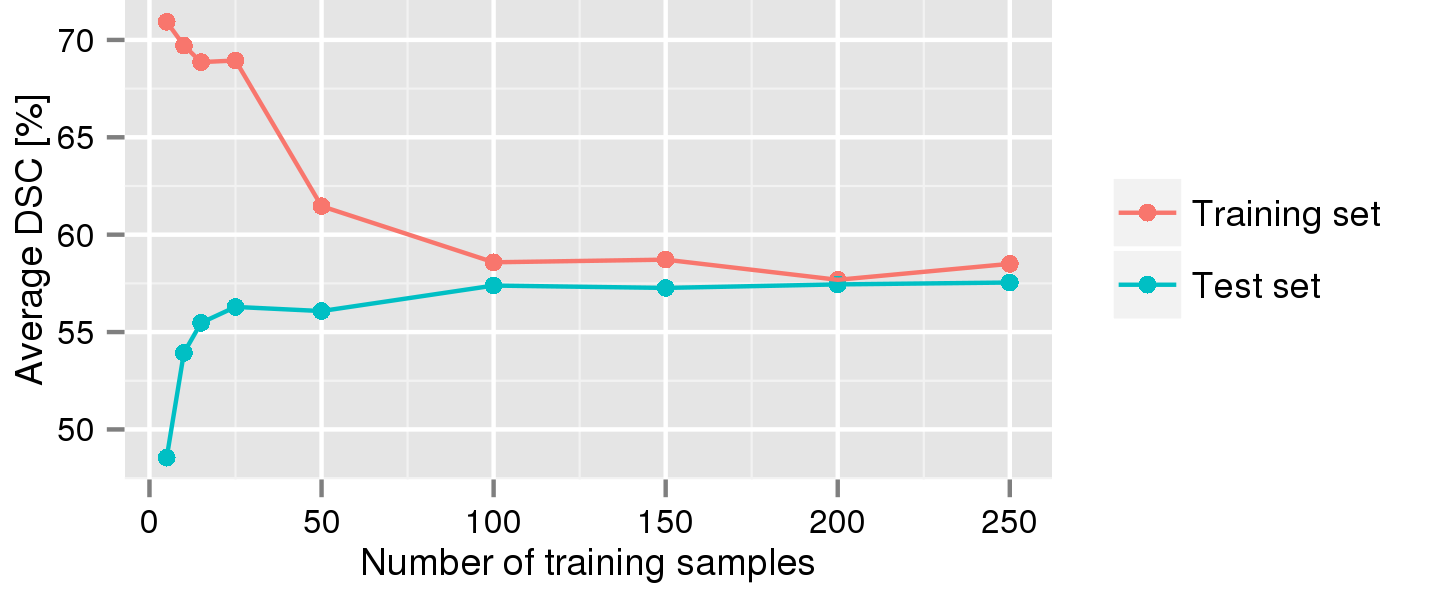
\includegraphics[width=0.78\textwidth]{figures/MICCAI2015_train_count}

\caption[Comparison of DSC scores calculated on the training and test sets for
varying numbers of training samples]{Comparison of DSC scores calculated on the training and test sets for
varying numbers of training samples. At around 100 samples, the model becomes
stable in terms of test performance and the small difference between training
and test DSCs, indicating that overfitting of the training data no longer
occurs.}
\label{fig:bioms}
\end{figure}

\section{Evaluation on In-house Data}

We evaluated the proposed method on a large data set from a multi-center MS
clinical trial. The data set, acquired from 67 different scanning sites,
consists of 377 pairs of FLAIR and T1-weighted MRIs from 195 subjects with a
resolution of \num{256x256x60} voxels and a voxel size of
\SI{0.936x0.936x3.000}{\milli\metre}. All images were skull-stripped using the
brain extraction tool (BET) \cite{jenkinson2005bet2}, followed by an intensity
normalization to the interval $[0,1]$, and a 6 degrees-of-freedom intra-subject
registration. To speed-up the training, all images were cropped to a
\num{164x206x52} voxel region-of-interest with the brain roughly centered. The
ground truth segmentations were produced using an existing semiautomatic 2D
region-growing technique, which has been used successfully in a number of large
MS clinical trials (e.g., \cite{kappos2006long} and
\cite{traboulsee2008reduction}). To carry out the segmentation, each lesion was
manually identified by a trained technician and then interactively grown from
the seed point. We used 300 image pairs for pre-training and fine-tuning, and
the remaining 77 image pairs for evaluation. Pre-training and fine-tuning were
performed using highly optimized GPU-accelerated implementations of 3D convRBMs
and CENs that were developed in-house \cite{brosch2014efficient}. Each model was
trained using 500 epochs. Pre-training and fine-tuning of a 7-layer CEN-s took
approximately 27 hours and 37 hours, respectively, on a single GeForce GTX 780
graphics card. However, once the network is trained, new image pairs can be
segmented in less than one second. We compared our results to the lesion masks
produced by Lesion-TOADS \cite{shiee2010topology}, a widely used freely
available tool for the fully automatic segmentation of MS lesions.

\subsection{Measures of Segmentation Accuracy}

We have used three different measures to evaluate segmentation accuracy. The
primary measure of accuracy that we employ is the Dice similarity coefficient
(DSC) \cite{dice1945measures}, which computes a normalized overlap value between
the produced and ground truth segmentations, and is defined as
\begin{equation}
\text{DSC} = \frac{2 \times \text{TP}}{2 \times \text{TP} + \text{FP} +
\text{FN}},
\end{equation}
where TP, FP, and FN denote the number of true positives, false positives, and
false negatives, respectively. A value of \SI{100}{\percent} indicates a perfect
overlap of the produced segmentation and the ground truth.
The DSC incorporates measures of over- and undersegmentation into a single
metric, which makes it a suitable measure to compare overall segmentation
accuracy.
In addition, we have used the true positive rate (TPR) and the positive
predictive value (PPV) to provide further information on specific aspects of
segmentation performance. The TPR is used to measure the fraction of the lesion
regions in the ground truth that are correctly identified by
an automatic method. It is defined as
\begin{equation}
\text{TPR} = \frac{\text{TP}}{\text{TP} + \text{FN}},
\end{equation}
where a value of \SI{100}{\percent} indicates that all true lesion voxels are
correctly identified. The PPV is used to determine the extent of the regions
falsely classified as lesion by an automatic method. It is defined as the
fraction of true lesion voxels out of all identified lesion voxels
\begin{equation}
\text{PPV} = \frac{\text{TP}}{\text{TP} + \text{FP}},
\end{equation}
where a value of \SI{100}{\percent} indicates that all voxels that are
classified as lesion voxels are indeed lesion voxels as defined by the ground
truth.

\subsection{Comparison of Network Architectures}

To determine the effect of network architecture, we compared the segmentation
performance of three different networks with each other and with Lesion-TOADS.
Specifically, we trained a 3-layer CEN and two 7-layer CENs, one with shortcut
connections and one without, on the 300 training pairs. The parameters of the
networks are given in Table~\ref{tab:arch3} and Table~\ref{tab:arch7}.
A comparison of the segmentation accuracy of the trained networks and
Lesion-TOADS is summarized in Table~\ref{tab:results1}. All CEN architectures
performed significantly better than Lesion-TOADS in overall segmentation
accuracy, where the improvements of the mean DSC scores range from 9\,pts for
the 3-layer CEN to 14\,pts for the 7-layer CEN with shortcut connections. The
improved segmentation performance is mostly due to a reduction of the false
positives. Lesion-TOADS achieved a mean PPV of only \SI{39.86}{\percent},
whereas the CEN with shortcut achieved a mean PPV of \SI{66.58}{\percent}---an
improvement of 27\,pts. The mean TPRs were roughly the same (slightly less than
\SI{50}{\percent}) for all methods except for the 7-layer CEN with shortcut,
which performed slightly better than the other methods with a mean TPR of
\SI{52.75}{\percent}.

Furthermore, the first experiment showed that increasing the depth of the CEN
and adding the shortcut connections improves the segmentation accuracy.
Increasing the depth of the CEN from three layers to seven layers improved the
mean DSC by 2\,pts. The improvement was confirmed to be statistically
significant using a one-sided paired $t$-test ($p\text{-value}=\num{0.002}$).
Adding a shortcut to the network further improved the segmentation
accuracy as measured by the DSC by 3\,pts. A second one-sided paired $t$-test
was performed to confirm the statistical significance of the improvement with a
$p$-value of \num{1.566e-11}.

% \begin{itemize}
% \item We used 3 different architectures: 3-layer, 7-layer without shortcuts and
% 7-layer with shortcuts.
% \item 7-layer CEN parameters are summarized in Table~\ref{tab:arch7}.
% \item Comparison of segmentation performance on the test set with 3 different
% architectures and lesionTOADS is shown in Table~\ref{tab:results1}
% \item Even the 3-layer model performs much better than lesionTOADS on average.
% \item Better was confirmed using a one-sided paired t-test. Give the p-value.
% \item Better than lesionTOADS ($p$-value = \num{4.732e-9})
% \item Better than 3-layer ($p$-value = \num{0.002})
% \item Better with shortcut connections ($p$-value = \num{1.566e-11})
% \item Adding more layers also improves performance. T-test.
% \item Adding shortcut connections improves performance. t-test.
% \end{itemize}

\begin{table}[tb]
\caption{Parameters of the 3-layer CEN used to evaluate different training
methods.}
\label{tab:arch3}
\centering
\begin{tabular}{@{}lccr@{}}
\toprule
Layer type & Kernel Size & \#Filters & \multicolumn{1}{c}{Image Size} \\
\midrule
Input & --- & --- & \num{164x206x52x2}\phantom{0} \\
Convolutional & \num{9x9x5x2} & 32 & \num{156x198x48x32} \\
Deconvolutional & \num{9x9x5x32} & 1 & \num{164x206x52x1}\phantom{0} \\
\bottomrule
\end{tabular}
\end{table}

\begin{table}[tb]
\caption{Parameters of the 7-layer CEN-s used to evaluate different training
methods.}
\label{tab:arch7}
\centering
\begin{tabular}{@{}lccr@{}}
\toprule
Layer type & Kernel Size & \#Filters & \multicolumn{1}{c}{Image Size} \\
\midrule
Input & --- & --- & \num{164x206x52x2}\phantom{0} \\
Convolutional & \num{9x9x5x2} & 32 & \num{156x198x48x32} \\
Average Pooling & \num{2x2x2} & --- & \num{78x99x24x32} \\
Convolutional & \num{9x10x5x32} & 32 & \num{70x90x20x32} \\
Deconvolutional & \num{9x10x5x32} & 32 & \num{78x99x24x32} \\
Unpooling & \num{2x2x2} & --- & \num{156x198x48x32} \\
Deconvolutional & \num{9x9x5x32} & 1 & \num{164x206x52x1}\phantom{0} \\
\bottomrule
\end{tabular}
\end{table}

\begin{table}
\begin{center}
\caption{Comparison of the segmentation accuracy of different CEN models with
Lesion-TOADS}
\label{tab:results1}
\begin{tabular}{@{}lccc@{}}
\toprule
Method & TPR [\%] & PPV [\%] & DSC [\%] \\
\midrule
3-layer CEN \cite{brosch2015} & \num{49.62+-20.32} & \num{59.87+-20.95} &
\num{49.1+-15.78} \\
7-layer CEN & \num{49.94+-19.96} & \num{63.5+-20} & \num{51.04+-14.71} \\
7-layer CEN-s & \num{52.75+-20.31} & \num{66.58+-20.71} &
\num{54.02+-15.24}
\\[0.2em]
Lesion-TOADS \cite{shiee2010topology} & \num{49.83+-14.79} & \num{39.86+-20.95} &
\num{40.04+-14.86} \\
\bottomrule
\end{tabular}
\end{center}
Note: The table shows the mean and standard deviation of the true positive rate
(TPR), positive predictive value (PPV), and Dice similarity coefficient (DSC).
\end{table}

\subsection{Comparison for Different Lesion Loads}

To examine the effect of lesion load on segmentation performance, we have
stratified the test set into five groups based on their reference lesion loads
as summarized in Table~\ref{tab:groups}. Most segmentation performance measures
deteriorate with lower lesion loads, because when there are only a few true
lesion voxels, even small segmentation errors can translate into large relative
errors. A comparison of segmentation accuracy of a 3-layer CEN and a 7-layer CEN
with shortcut for different lesion loads is illustrated in
Fig.~\ref{fig:l1vl2}. Adding four layers and shortcut connections improves the
segmentation accuracy for all lesion load groups, where the improvements are
largest for the highest lesion loads. In MS, lesion load is strongly
correlated with lesion size, which means that the group with the highest lesion
load also contains scans with the largest lesions. The receptive field of the
3-layer CEN has a size of only \num{17x17x9} voxels, which reduces its ability
to identify very large lesions. In contrast, the 7-layer CEN has a receptive
field size of \num{49x53x26} voxels, which allows it to learn features that can
capture much larger lesions than the 3-layer CEN. Consequently, the 7-layer CEN
is able to learn a feature set that captures a wider range of lesion sizes,
which in turn improves the segmentation accuracy especially for very high lesion
loads, where larger lesions are also more prevalent.

\begin{table}[tb]
\caption[Lesion load classes as used for the detailed analysis]{Lesion load
classes as used for the detailed analysis.}
\label{tab:groups}
\begin{center}
\begin{tabular}{@{}lcc@{}}
\toprule
Group & Lesion load in \si{\cubic\milli\metre} & Number of samples \\
\midrule
% 0, 1250, 2500, 3800, 10000
Very low & $[0,3250]$ & 17 \\
Low      & $(3250,6500]$ & 16 \\
Medium & $(6500,10000]$ & 18 \\
High & $(10000,25000]$ & 18 \\
Very high & $> 25000$ & 8 \\
\bottomrule
\end{tabular}
\end{center}
\end{table}

% \begin{itemize}
% \item Analyse where the performance gains come from
% \item 7-layer CEN improves across the board but improvements are particularly
% high for large lesion loads
% \item Large lesion load is also associated with larger lesions
% \item Small filters fail to detect large lesions correctly
% \item 7-layer CEN uses a hierachy of features where each layer represents
% features of a different scale
% \item This allows the detection of a wider spectrum of lesion sizes.
% \item Analyse the relationship of segmentation performance and lesion load
% \item Divided the test set into 5 classes with roughly the same number of
% samples. Classes are (0,1250) ($n=17$), (1250,2500) ($n=16$), (2500, 3800)
% ($n=18$), (3800,10000) ($n=18$), above 10000 ($n=8$). Mention the number of
% samples per class.
% \item CEN outperforms Lesion-TOADS for all lesion load categories, except for
% very high lesion load.
% \item For very high lesion load, no difference to Lesion-TOADS found using
% t-test.
% \item TPR, PPV, DSC for different lesion loads in a table.
% \end{itemize}

\begin{figure}[tb]
\centering
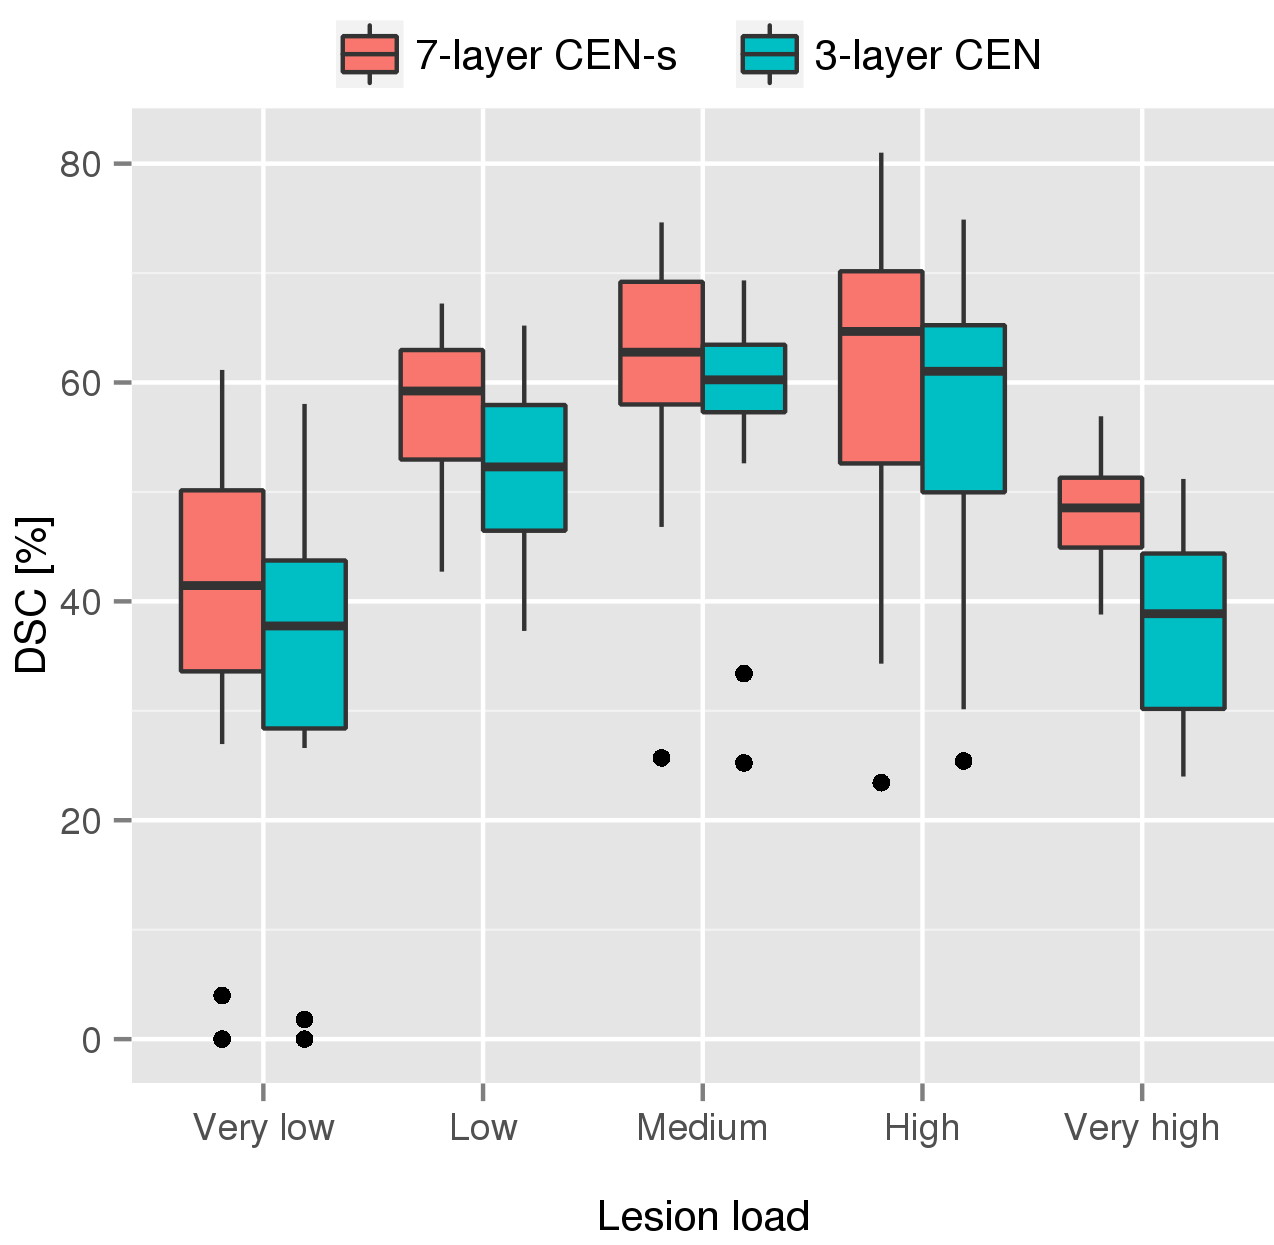
\includegraphics[width=\columnwidth]{figures/TMI_boxplot_L1vsL2}

\caption[Comparison of the segmentation accuracy of a 3-layer CEN and a
7-layer CEN-s for different lesion load groups]{Comparison of the segmentation
accuracy (DSC) of a 3-layer CEN and a 7-layer CEN-s for different lesion load groups. Adding four layers and
shortcut connections improves the performance across all lesion loads, where the
improvements are especially large for scans with large lesion loads, which are
also correlated with lesion size.}

\label{fig:l1vl2}
\end{figure}

% TODO: The small number of scans in the highest load group makes comparing
% across groups difficult. Maybe weaken the statement or point out the
% limitation with sample size.

Fig.~\ref{fig:l2vlt} shows a comparison of the 7-layer CEN with shortcut and
Lesion-TOADS. The CEN approach performs more consistently than Lesion-TOADS for
all lesion load groups, but the greatest improvements are for very low to medium
lesion loads. For the group with very high lesion loads, Lesion-TOADS achieves a
slightly higher mean DSC than the CEN approach, but the difference is very small
compared to the gains in accuracy achieved by the CEN for the other lesion load
groups.
% However, a two-sided paired $t$-test yielded that
% the difference is not statistically significant ($p\text{-value}=0.2566$).
Table~\ref{tab:result2} shows a more detailed
comparison. While the PPV increases consistently with higher lesion loads for
both methods, the TPR is highest for low to medium lesion loads and decreases
again for high to very high lesion loads. This shows the difficulty for both
methods to correctly identify very large lesions that can extend far into the
white matter.

\begin{figure}[tb] \centering
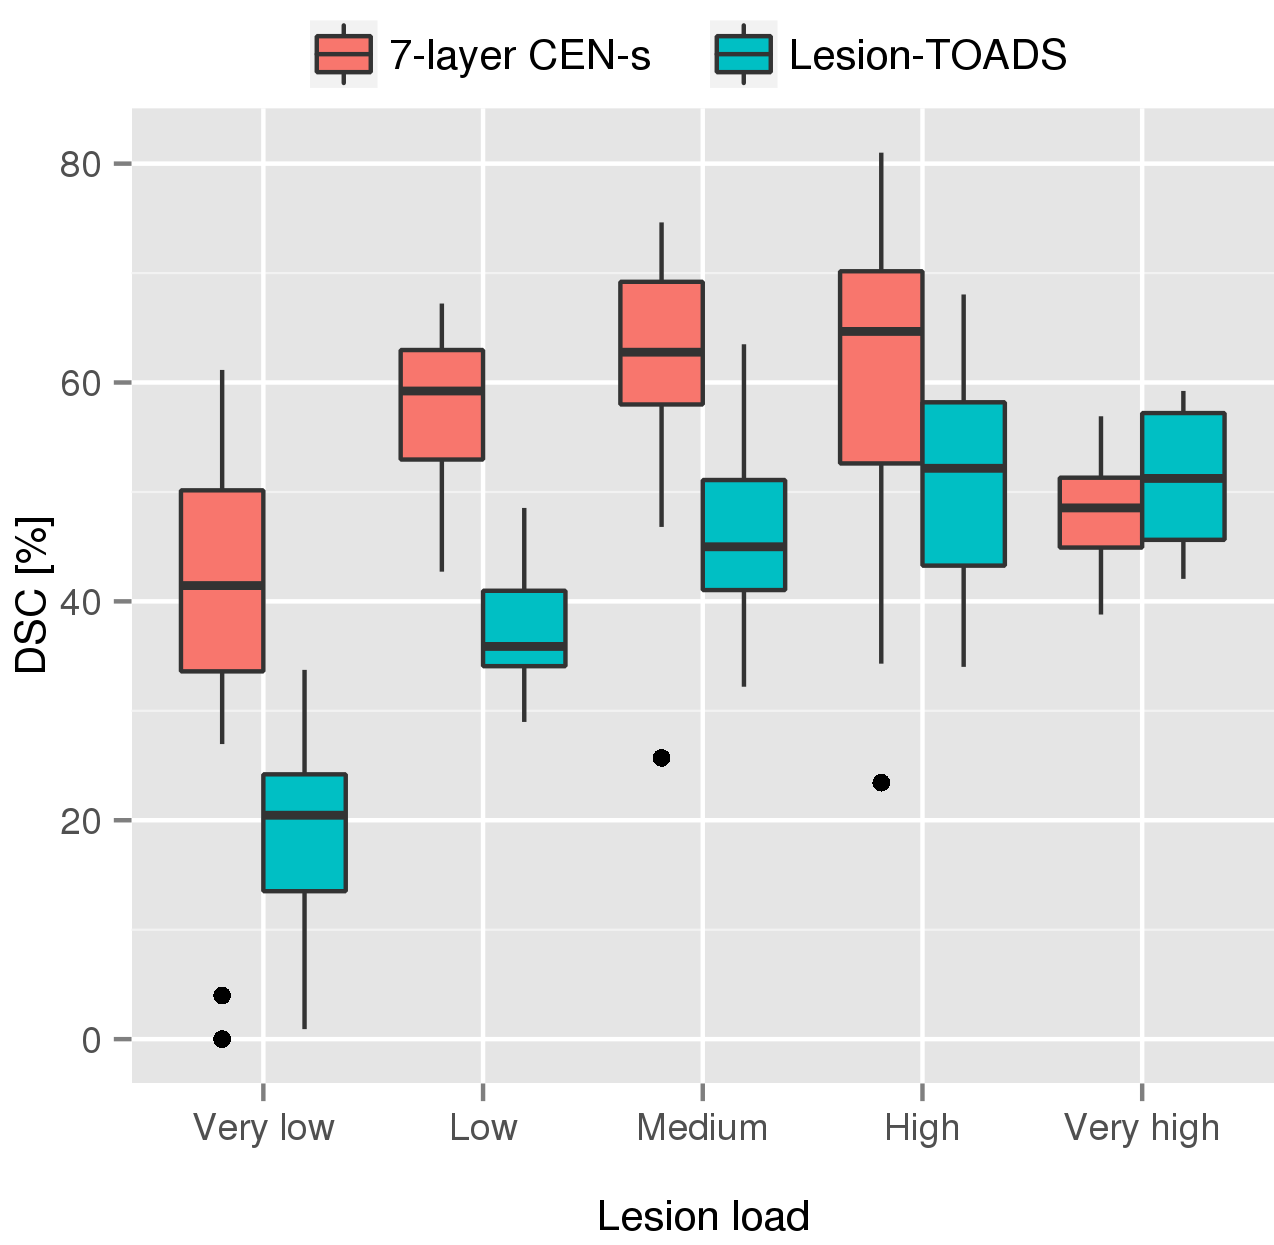
\includegraphics[width=\columnwidth]{figures/TMI_boxplot_LTvsL2}
\caption[Comparison of the segmentation accuracy of Lesion-TOADS and a 7-layer
CEN with shortcut connections for different lesion loads]{Comparison of the
segmentation accuracy (DSC) of Lesion-TOADS and a 7-layer CEN with shortcut
connections for different lesion loads. The CEN approach is much more sensitive
in detecting small lesions, while still being able to detect large lesions.}
\label{fig:l2vlt}
\end{figure}

\begin{table}
\caption{Comparison of segmentation accuracy for different lesion load
categories.}
\label{tab:result2}
\begin{center}
\begin{tabular}{@{}lcccccc@{}}
\toprule
\multicolumn{1}{@{}l}{Lesion load} & \multicolumn{3}{c}{7-layer CEN-s} &
\multicolumn{3}{c@{}}{Lesion-TOADS}
\\
& TPR & PPV & DSC & TPR & PPV & DSC \\
\midrule
% \phantom{000}$(0,1250]$\phantom{0} & \num{50.00} & \num{41.15} & \num{39.34} &
% \num{49.96} & \num{13.09} & \num{18.86}\\
% $(1250,2500]$\phantom{0} & \num{61.92} & \num{59.01} & \num{57.45} & \num{52.39}
% & \num{29.95} & \num{37.74}\\
% $(2500,3800]$\phantom{0} & \num{57.64} & \num{71.54} & \num{61.31} & \num{54.17}
% & \num{41.83} & \num{46.53}\\
% $(3800,10000]$ & \num{51.14} & \num{81.11} & \num{60.13} & \num{47.97} &
% \num{56.56} & \num{50.76}\\
% $> 10000$ & \num{32.82} & \num{91.95} & \num{48.19} & \num{38.88} & \num{74.6} &
% \num{50.93}\\
Very low & \num{50.00} & \num{41.15} & \num{39.34} &
\num{49.96} & \num{13.09} & \num{18.86}\\
Low & \num{61.92} & \num{59.01} & \num{57.45} & \num{52.39}
& \num{29.95} & \num{37.74}\\
Medium & \num{57.64} & \num{71.54} & \num{61.31} & \num{54.17}
& \num{41.83} & \num{46.53}\\
High & \num{51.14} & \num{81.11} & \num{60.13} & \num{47.97} &
\num{56.56} & \num{50.76}\\
Very high & \num{32.82} & \num{91.95} & \num{48.19} & \num{38.88} & \num{74.6} &
\num{50.93}\\
\bottomrule
\end{tabular}
\end{center}
\end{table}

% \begin{itemize}
% \item Have some sample images and discuss what we can see here.
% \end{itemize}

\subsection{Qualitative Results}

A qualitative comparison of segmentation performance for four characteristic
cases is shown in Fig.~\ref{fig:images}. Our method uses a combination of
automatically learned intensity and appearance features, which makes it
inherently robust to noise (see Fig.~\ref{fig:images}a), while still being able
to detect small isolated lesions (see Fig.~\ref{fig:images}b). Furthermore, our
method is able to learn a wide spectrum of lesion shapes and appearances from
training data, which allows our method to correctly identify multiple different
types of MS lesions. For example, our method was able to correctly identify the
T1 black hole shown in Fig.~\ref{fig:images}c, which present a known limitations
of Lesion-TOADS \citep{shiee2010} and was partially missed.
Figure~\ref{fig:images}d shows one of the most challenging cases for our method.
Very large lesions can extend beyond the size of the receptive field of the CEN,
which reduces its ability to extract characteristic lesion features.
Consequently, in some cases our method can underestimate the size of very large
lesions.

\begin{figure}
%\centering
\hspace*{-5pt}
\subfloat[Robust to noise] {
\begin{tikzpicture}[node distance=1.5cm and 0.1\columnwidth,
  font=\footnotesize, on grid]
  
\node[inner sep=0] (image) {
  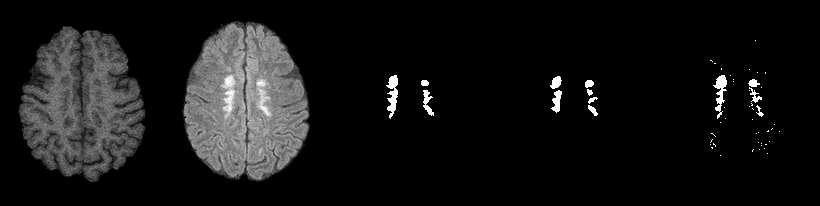
\includegraphics[width=0.5\columnwidth]{figures/TMI_p15s34_robust_to_noise3}
  }; \node[above=of image] (gt) {\phantom{g}Ground truth\phantom{g}};
\node[left=of gt] (flair) {\phantom{g}FLAIR\phantom{g}};
\node[left=of flair] {T1-weighted};
\node[right=of gt,align=center] (cen) {\phantom{g}Our method\phantom{g}};
\node[right=of cen,align=center] {Lesion-\\ TOADS};


\end{tikzpicture}
}
\subfloat[Can detect small isolated lesions.] {
\begin{tikzpicture}[node distance=1.5cm and 0.1\columnwidth,
  font=\footnotesize, on grid]
  
\node[inner sep=0] (image) {
  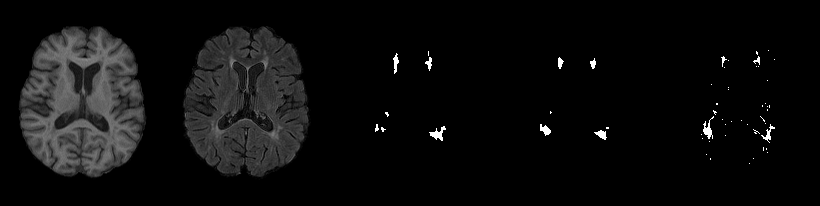
\includegraphics[width=0.5\columnwidth]{figures/TMI_p17s29_noisy_lesionTOADS}};
  \node[above=of image] (gt) {\phantom{g}Ground truth\phantom{g}};
\node[left=of gt] (flair) {\phantom{g}FLAIR\phantom{g}};
\node[left=of flair] {T1-weighted};
\node[right=of gt,align=center] (cen) {\phantom{g}Our method\phantom{g}};
\node[right=of cen,align=center] {Lesion-\\ TOADS};

\draw[green, thick] (-7pt,-3.5pt) circle (3pt);
\begin{scope}[xshift=0.1\columnwidth]
\draw[green, thick] (-7pt,-3.5pt) circle (3pt);
\end{scope}

\end{tikzpicture}
}\\
\hspace*{-5pt}
\subfloat[Example of a T1 black hole that was correctly identified by our
method.] {
\begin{tikzpicture}
\node[inner sep=0pt] {
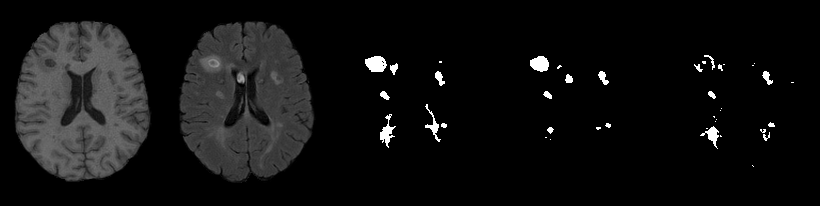
\includegraphics[width=0.5\columnwidth]{figures/TMI_p36s30_blackhole}};
\draw[red,thick] (-10pt,12pt) circle (7pt);
\begin{scope}[xshift=-0.1\columnwidth]
\draw[red,thick] (-10pt,12pt) circle (7pt);
\end{scope}
\begin{scope}[xshift=-0.2\columnwidth]
\draw[red,thick] (-10pt,12pt) circle (7pt);
\end{scope}
\begin{scope}[xshift=0.1\columnwidth]
\draw[red,thick] (-10pt,12pt) circle (7pt);
\end{scope}
\begin{scope}[xshift=0.2\columnwidth]
\draw[red,thick] (-10pt,12pt) circle (7pt);
\end{scope}
\end{tikzpicture}
}
\subfloat[Very large lesions can be underestimated] {
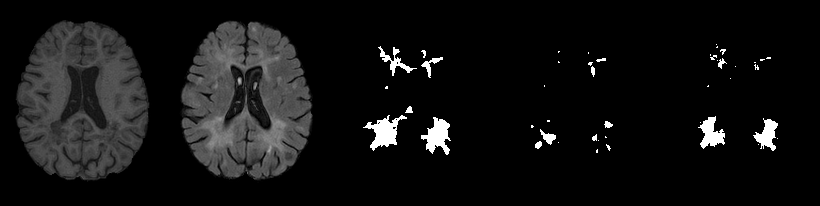
\includegraphics[width=0.5\columnwidth]{figures/TMI_p54s32_large_lesions}
}

\caption[Four cases illustrating the strengths and limitations of our method
compared to Lesion-TOADS]{Four cases illustrating the strengths and limitations
of our method compared to Lesion-TOADS. Our method is inherently robust to noise
(a), while still being able to detect small isolated lesions (b). Furthermore,
our method is able to detect multiple different types of lesions correctly
(e.g., T1 black holes). However, in some cases our method can underestimate the
size of very large lesions (d).}

\label{fig:images}
\end{figure}
